\documentclass{beamer}

\usetheme{Padova}

\title{Sentiment Analysis on Online Automotive Forums}
%\subtitle{Curabitur sit amet mi magna}
\author[me]{\vspace{5mm}\textit{Candidate}: Giuseppe Ravagnani\\\textit{Supervisor}: Prof. Nicola Ferro\\\textit{Co-Supervisor}: Davide Lappon\\[5mm]}

\date{September 30, 2019}


\begin{document}

	\maketitle

%	\begin{frame}{Outline}
%		\tableofcontents
%	\end{frame}


	\section{Motivation}
	
	\begin{frame}{Motivation}
		\begin{columns}
			\column{0.5\textwidth}
			\centering
			\begin{figure}
				
\includegraphics[width=.9\linewidth]{figures/reply2.pdf}
			\end{figure}
			\column{0.5\textwidth}
			\centering
			\begin{figure}
				
\includegraphics[width=.6\linewidth]{figures/porsche2.png}
			\end{figure}
		\end{columns}
	\end{frame}
	
	

%	\begin{frame}{Introduction (1)}
%
%		\textit{Sentiment Analysis} is an active area of research in Natural Language Processing, motivated to improve the automated recognition of sentiment expressed in text \vspace{.5em}
%
%		\begin{itemize}
%			\item From the whole scenic of online social media, Twitter is the most used to achieve
%			contents \vspace{.5em}
%			\item Most existing techniques for sentiment classification involve supervised learning \vspace{.5em}
%			\item Used for collecting people's sentiment information about a given topic
%		\end{itemize}
%	\end{frame}

%	\begin{frame}{Introduction (2)}
%		
%		\begin{itemize}
%			\item[$\rightarrow$] \textbf{Dataset}: the need of a set of already annotated data for applying machine learning models
%			\item[$\rightarrow$] \textbf{Development}:
%				\begin{itemize}
%					\item Twitter Sentiment Analysis Algorithm
%					\item Relevance Detection for class "Engine"
%					\item Sentiment Classification for class "Engine"
%					\item Cascade Classifier
%				\end{itemize}
%			\item[$\rightarrow$] \textbf{Goal}: Develop an aspect-based sentiment analysis tool in automotive field for a specific brand	
%			\item[$\rightarrow$] \textbf{Collaboration}: Reply Technology for commission of Porsche
%		\end{itemize}
%	
%	\end{frame}


	\section{Why}
	
%	\begin{frame}
%		perchè io e non qualcosa che esiste gia (dominio specifico, italiano, slide tweet e forum)
%	\end{frame}

	
	
	\begin{frame}{Automotive Forums vs Twitter}
		
		\begin{exampleblock}{Example Twitter}
			\fbox{@united} I do not see where it talks about military baggage fees. Can you please guide me. Thanks \fbox{\#usairline}
		\end{exampleblock}
		
		\begin{exampleblock}{Example Automotive Forum}
			{\scriptsize
				Sono reali calcolati nel arco del tutto anno nel estate qualcosa in più causa
				gomme di 17” e climatizzatore nel inverno un po di meno. Per quanto
				riguarda le autostrade quelle che percorro io principalmente la A4 e molto
				congestionata cosi spesso la media e \fbox{110-115 km/h} che ovviamente influisce
				positivamente a i consumi. Ma quello che mi piace di più è assenza dei
				guasti. Sulla vecchia \fbox{Accord} il primo guasto lo ho avuto a \fbox{200000 km} si è
				rotto il termostato della clima. Ogni tanto faccio giro di altri forum e leggo
				delle turbine rotte catene di distribuzione progettate male iniettori fatti male
				mah nel 2015 per me sono le cose incomprensibili. Con tutti gli difetti che
				può avere preferisco la \fbox{Honda}.}
		\end{exampleblock}
		
	\end{frame}




	\section{Sentiment Analysis Algorithms}
	
%	\begin{frame}{State of the Art Algorithms}
%		
%		From: Zimbra, David \& Abbasi, Ahmed \& Zeng, Daniel. (2018).\\ The State-of-the-Art in Twitter Sentiment Analysis:\\ A Review and Benchmark Evaluation.
%		
%		\begin{table}
%			\centering
%			\scriptsize
%			\begin{tabular}{| c || c | c | c | c | c | c || c |}
%				\hline
%				& \textbf{Average} & \textbf{Pharma} & \textbf{Retail} & \textbf{Security} & \textbf{Tech} & \textbf{Telco} & \textbf{Ensemble}\\
%				\hline
%				\textbf{BPEF} & 71.38 & 67.81 & 65.24 & 75.32 & 76.30 & 72.21 & yes\\
%				\hline
%				\textbf{NRC} & 71.33 & 75.26 & 64.93 & 76.39 & 64.96 & 75.08 & no\\
%				\hline
%				\textbf{Webis} & 71.41 & 76.16 & 64.40 & 77.37 & 63.68 & 75.46 & yes\\
%				\hline
%			\end{tabular}
%		\end{table}
%	
%	\end{frame}





	\section{Dataset}
	
	\begin{frame}{Dataset Gathering}
		
		The creation of a suitable dataset is mandatory to train machine learning algorithm.
		\begin{itemize}
			\item Crawled some of the most visited Italian automotive forums (Quattroruote, Autopareri, Bmwpassion, HDmotori, Porschemania, Forumelettrico)
			\item Comments have been annotated with respect to the classes "Brand", "Interiors", "Exteriors", "Mechanics", "Performance", "Consumption", "Engine", "Electrical mobility", "Off-road" and "Technology", picking the labels "positive", "negative", "neutral"
			\item Relevance classification with an additional "irrelevant" label
			\item From a total of 1,200,000 crawled comments, a random subset of 7,183 have been manually annotated
		\end{itemize}
		
	\end{frame}
	
	
	\begin{frame}{Dataset Statistics}
		
		\only<1>{
			\begin{figure}
				\centering
				\vspace{-5mm}
				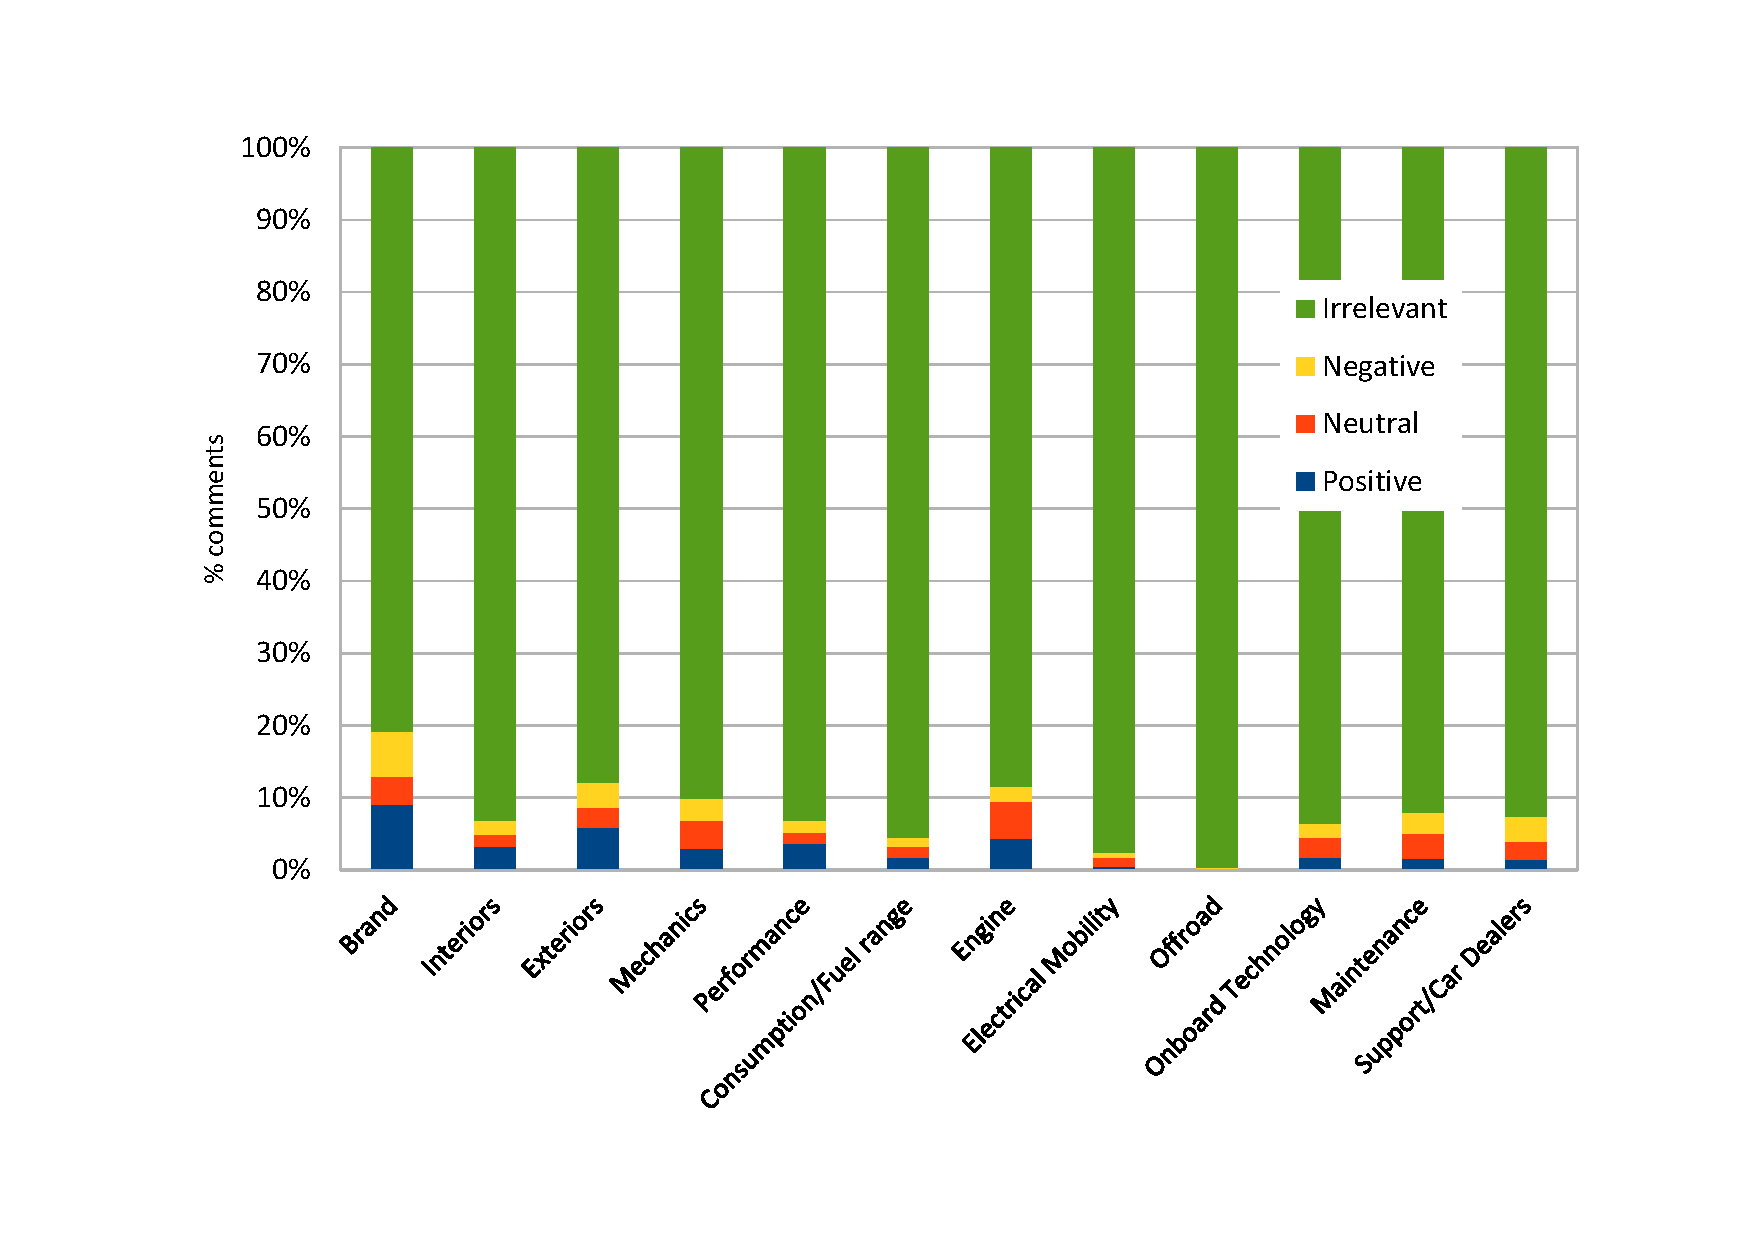
\includegraphics[width=\linewidth]{figures/stats1.pdf}
			\end{figure}
		}
		\only<2>{
			\begin{figure}
				\centering
				\vspace{-5mm}
				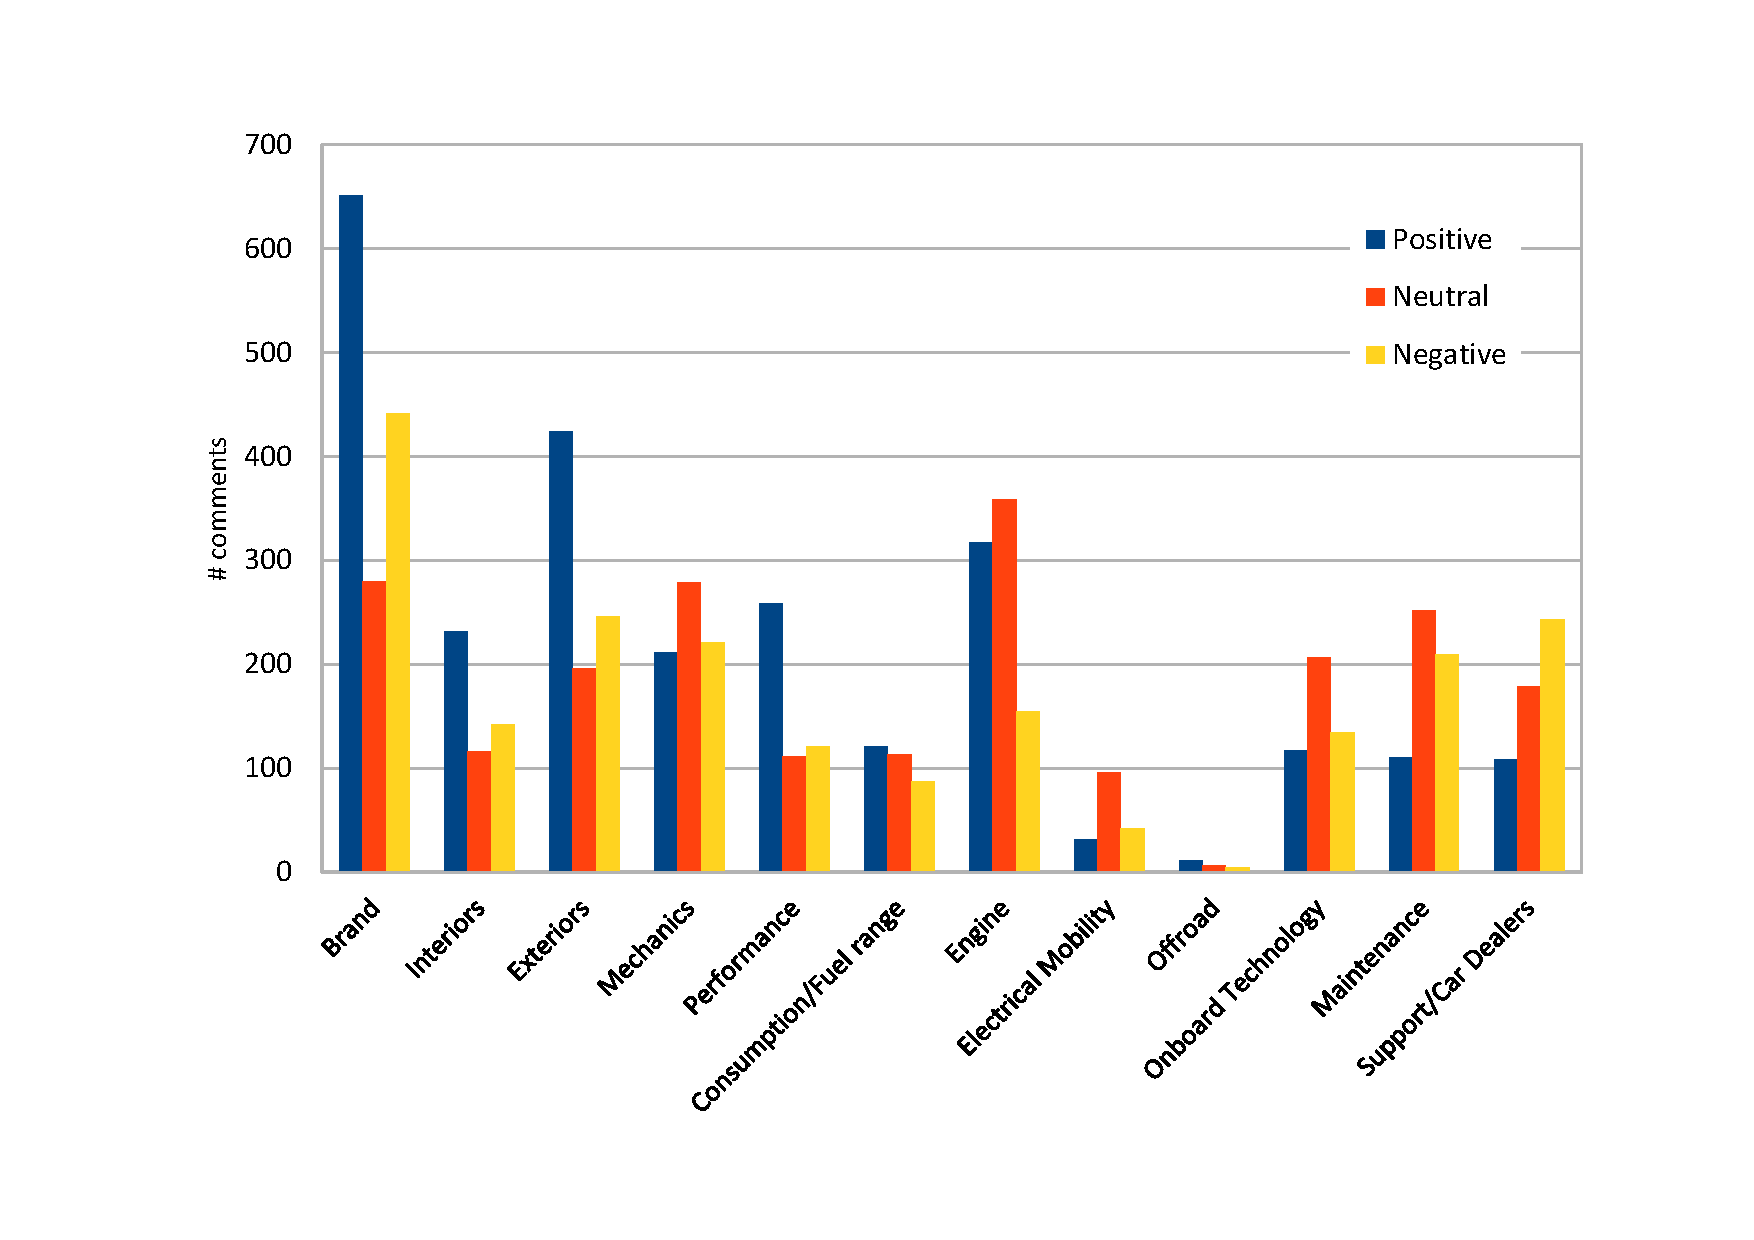
\includegraphics[width=\linewidth]{figures/stats2.pdf}
			\end{figure}
		}
		
	\end{frame}
	








%	\begin{frame}{Bootstrap Ensemble Framework (BPEF)}
%		
%		\begin{figure}
%			\centering
%			\vspace{-5mm}
%			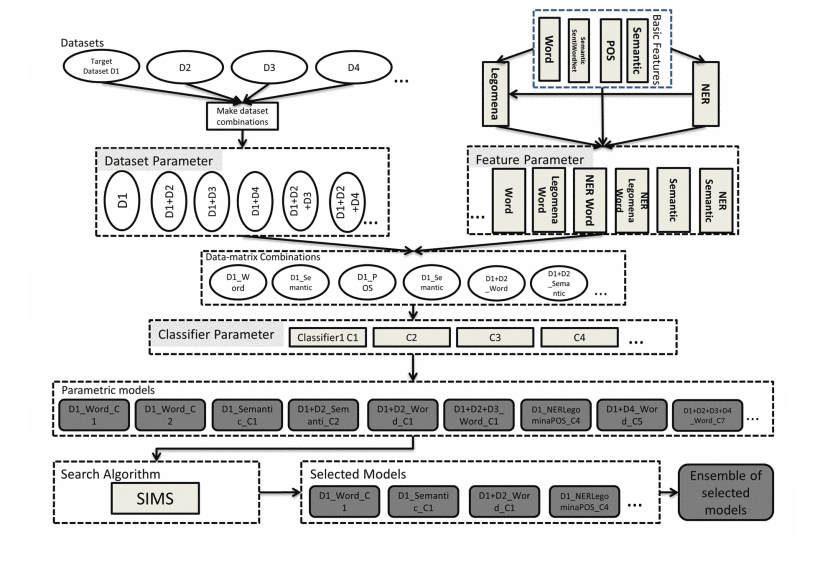
\includegraphics[width=\linewidth]{figures/bpef.png}
%		\end{figure}
%				
%	\end{frame}








	







	\section{My Implementation}

	\begin{frame}{Baseline algorithm}
		
		\begin{itemize}
%			\only<1>{
%				\item[$\rightarrow$] Twitter preprocessing:
%				\begin{enumerate}
%					\item lowercase, punctuation and stopwords removal
%					\item "http://someurl" $\rightarrow$ "URL"
%					\item "\#hashtag" $\rightarrow$ "hashtag"
%					\item happy emoticons $\rightarrow$ "EMO\_POS" \\sad emoticons $\rightarrow$ "EMO\_NEG"
%					\item stemming
%				\end{enumerate}
%			}
			\only<1>{
				\item[$\rightarrow$] Preprocessing:
				\begin{enumerate}
					\item encoding correction
					\item lowercase, punctuation and stopwords removal
					\item "http://someurl" $\rightarrow$ "URL"
					\item replacing domain-specific tokens with common string (distances, speed, consumption, weight, power, ...)
					\item stemming
				\end{enumerate}
			}
			\item[$\rightarrow$] Support Vector Machine (SVM) Classifier with Term Frequency - Inverse Document Frequency (TF-IDF) features vectorization
			\[tf_{i,j}=\frac{n_{i,j}}{|d_j|}, \quad idf_i=\log \frac{|D|}{|\{d:i\in d\}|}, \quad tf\text{-}idf_{i,j}=tf_{i,j} \times idf_i\]
		\end{itemize}
		
 	\end{frame}
 	
 	

	\begin{frame}{Bootstrap Ensemble Framework (BPEF)}
		
		\only<1>{
			\begin{figure}
				\centering
				%\vspace{-5mm}
				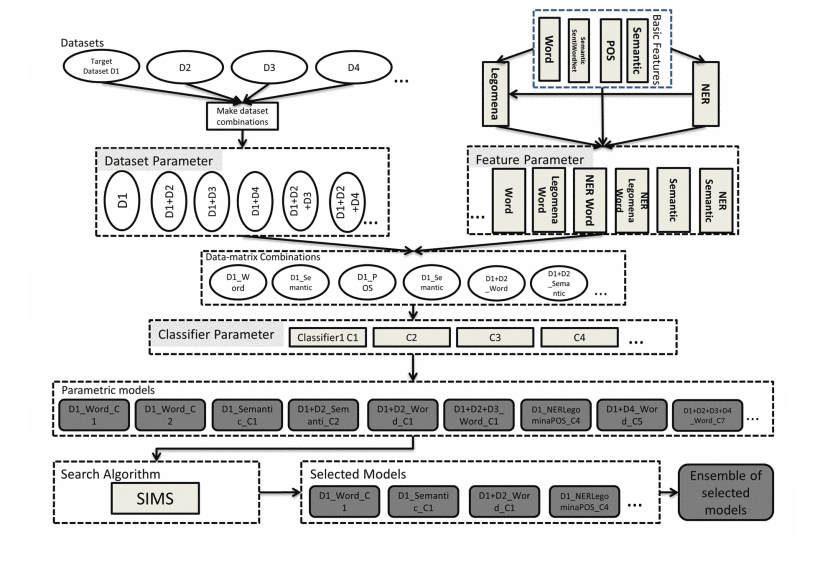
\includegraphics[width=\linewidth]{figures/bpef.png}
			\end{figure}
		}
		\only<2>{
			\begin{figure}
				\centering
				%\vspace{-5mm}
				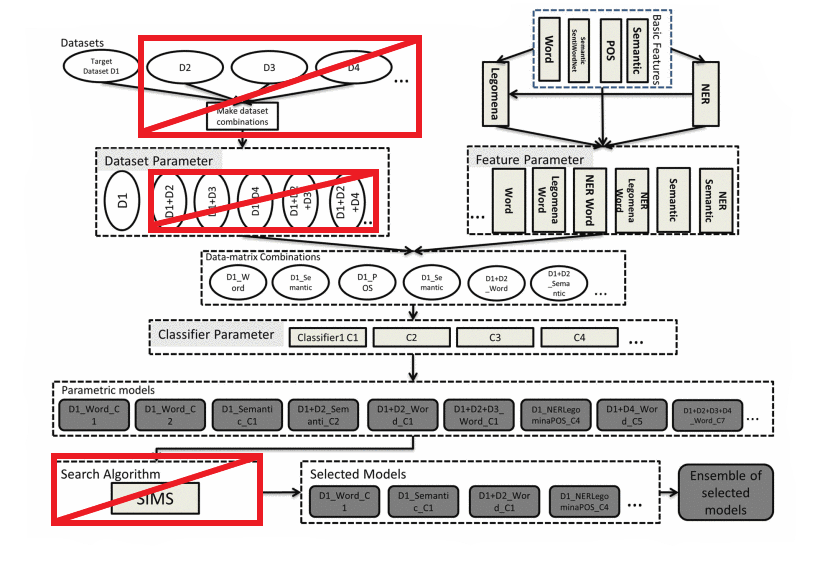
\includegraphics[width=\linewidth]{figures/my_bpef.png}
			\end{figure}
		}
		
	\end{frame}



	\begin{frame}{Cascade Classifier}
		
		Implementation of a cascade classifier for the four-label classification.
		
		\begin{figure}
				\centering
				%\vspace{-5mm}
				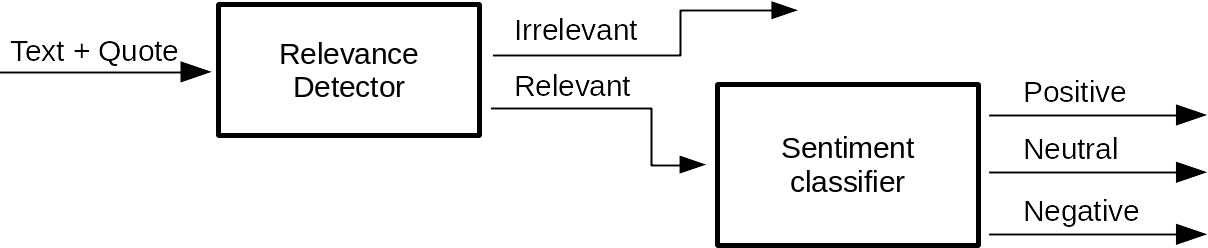
\includegraphics[width=\linewidth]{figures/blocks_cascade.png}
		\end{figure}
	
		\begin{itemize}
			\item Logistic Regression relevance detector
			\item BPEF Sentiment classifier
		\end{itemize}
		
		
	\end{frame}



	\section{Results}
	
%	\begin{frame}{Results: Tests on Twitter}
%		\begin{columns}
%			\column{0.5\textwidth}
%			\centering
%			Baseline\vspace{0.7cm}\\
%			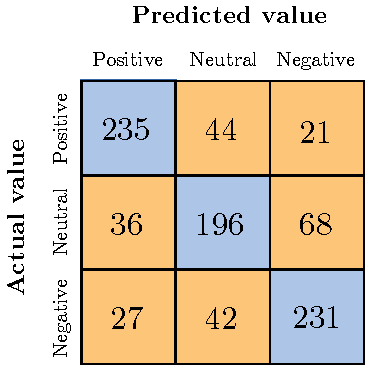
\includegraphics[width=0.7\linewidth]{figures/twitter_snt_svm_tst.pdf}\\
%			\begin{table}
%				\centering
%				\begin{tabular}{| c | c |}
%					\hline
%					\textbf{F-macro} & 0.735 \\
%					\hline
%					\textbf{Accuracy} & 0.736 \\
%					\hline
%				\end{tabular}
%			\end{table}
%			
%			\column{0.5\textwidth}
%			\centering
%			BPEF\vspace{0.7cm}\\
%			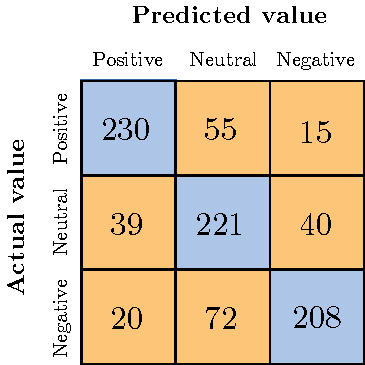
\includegraphics[width=0.7\linewidth]{figures/twitter_snt_bpef_tst.pdf}\\
%			\begin{table}
%				\centering
%				\begin{tabular}{| c | c |}
%					\hline
%					\textbf{F-macro} & 0.734 \\
%					\hline
%					\textbf{Accuracy} & 0.732 \\
%					\hline
%				\end{tabular}
%			\end{table}
%			
%			
%		\end{columns}
%	\end{frame}


	\begin{frame}{Results: Tests on our Dataset}
		
%		\only<1>{
%			\centering
%			\textbf{Relevance detection}\vspace{0.5cm}
%		
%			\begin{columns}
%				\column{0.5\textwidth}
%				\centering
%				SVM\vspace{0.7cm}\\
%				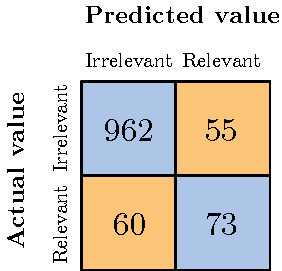
\includegraphics[width=0.6\linewidth]{figures/ita_rel_svm_afs.pdf}\\
%				\begin{table}
%					\centering
%					\begin{tabular}{| c | c |}
%						\hline
%						\textbf{F1-macro} & 0.559 \\
%						\hline
%						\textbf{Recall} & 0.570 \\
%						\hline
%						\textbf{Precision} & 0.549 \\
%						\hline
%					\end{tabular}
%				\end{table}
%				
%				\column{0.5\textwidth}
%				\centering
%				Logistic Regression\vspace{0.7cm}\\
%				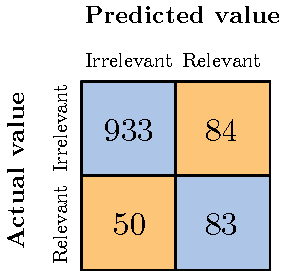
\includegraphics[width=0.6\linewidth]{figures/ita_rel_logreg_afs.pdf}\\
%				\begin{table}
%					\centering
%					\begin{tabular}{| c | c |}
%						\hline
%						\textbf{F1-macro} & 0.553 \\
%						\hline
%						\textbf{Recall} & 0.624 \\
%						\hline
%						\textbf{Precision} & 0.497 \\
%						\hline
%					\end{tabular}
%				\end{table}
%				
%				
%			\end{columns}
%		
%		}
		\only<1>{
			\centering
			\textbf{Sentiment classification}\vspace{0.5cm}
			
			\begin{columns}
				\column{0.5\textwidth}
				\centering
				SVM\vspace{0.7cm}\\
				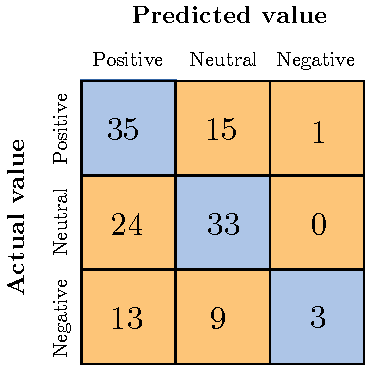
\includegraphics[width=0.6\linewidth]{figures/ita_snt_svm_afs.pdf}\\
				\begin{table}
					\centering
					\begin{tabular}{| c | c |}
						\hline
						\textbf{F1-macro} & 0.451 \\
						\hline
					\end{tabular}
				\end{table}
				
				\column{0.5\textwidth}
				\centering
				BPEF\vspace{0.7cm}\\
				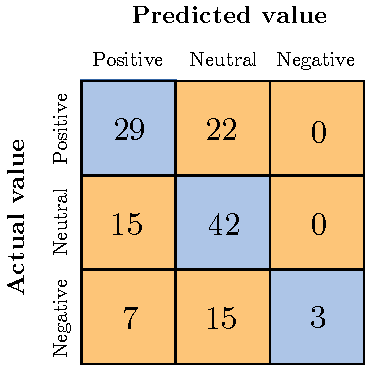
\includegraphics[width=0.6\linewidth]{figures/ita_snt_bpef_afs.pdf}\\
				\begin{table}
					\centering
					\begin{tabular}{| c | c |}
						\hline
						\textbf{F1-macro} & 0.467 \\
						\hline
					\end{tabular}
				\end{table}
				
				
			\end{columns}
			
		}
		\only<2>{
			
			\centering
			\textbf{4-labels classification}\vspace{0.5cm}
			
			\begin{columns}
				\column{0.5\textwidth}
				\centering
				SVM\vspace{0.7cm}\\
				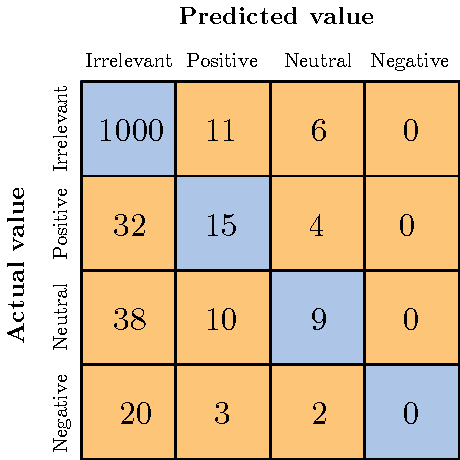
\includegraphics[width=0.6\linewidth]{figures/ita_4l_svm_afs.pdf}\\
				\begin{table}
					\centering
					\begin{tabular}{| c | c |}
						\hline
						\textbf{F1-macro} & 0.378 \\
						\hline
					\end{tabular}
				\end{table}
				
				\column{0.5\textwidth}
				\centering
				Cascade classifier\vspace{0.7cm}\\
				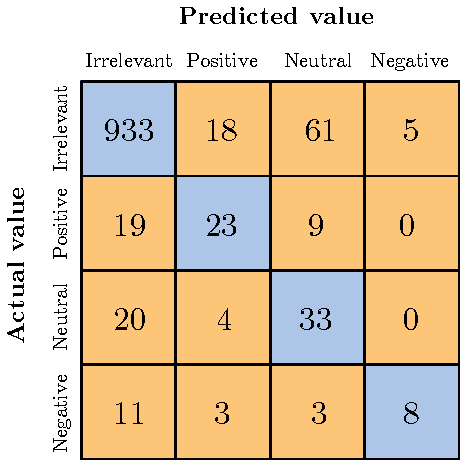
\includegraphics[width=0.6\linewidth]{figures/ita_cascade_bpef_val.pdf}\\
				\begin{table}
					\centering
					\begin{tabular}{| c | c |}
						\hline
						\textbf{F1-macro} & 0.556 \\
						\hline
					\end{tabular}
				\end{table}
				
				
			\end{columns}
			
		}
		
	\end{frame}







	
	\section{Data Visualization}
	
	\begin{frame}{Data Visualization}
		\centering
		\vspace{-5mm}
		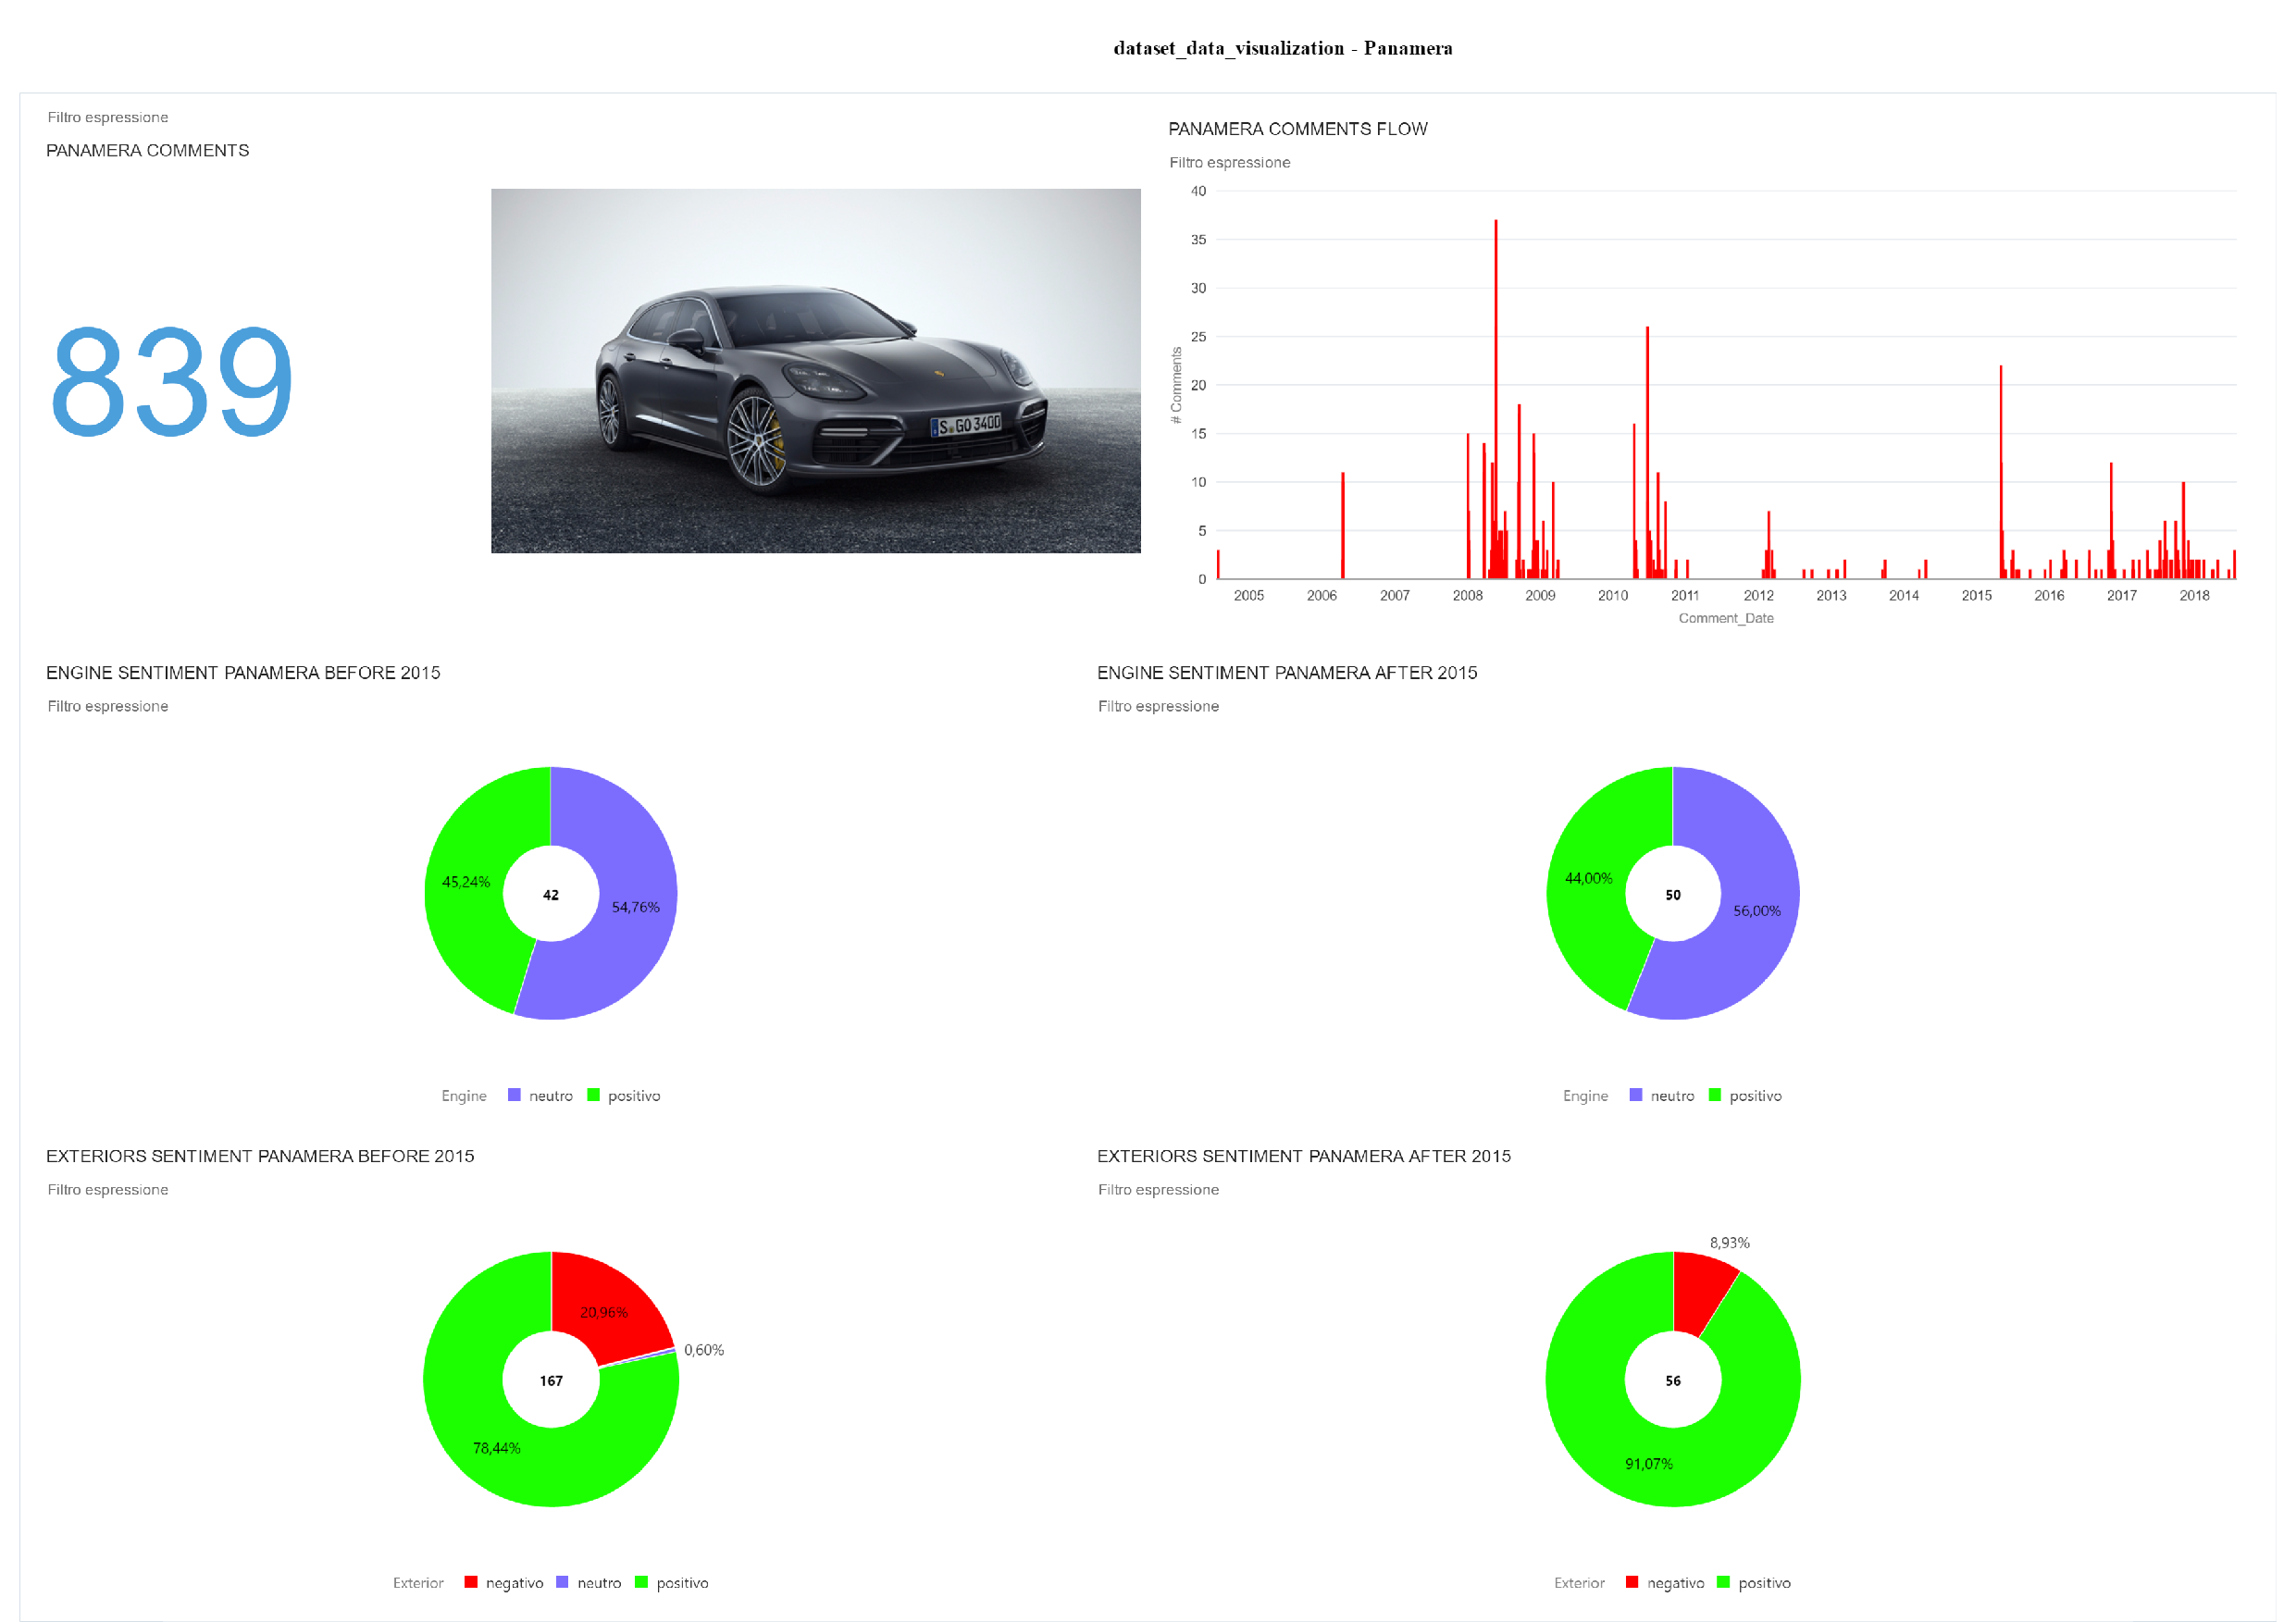
\includegraphics[width=\linewidth]{figures/dataset_data_visualization_2.pdf}

	\end{frame}









	\section{Conclusions \& Enhancements}
	
	\begin{frame}{Conclusions \& Future Works}
		
		\begin{itemize}
			\item BPEF model overcomes baseline approach
			\item Implemented model can be considered reliable for sentiment classification for Italian automotive forums
			\vspace{1cm}
			\item Expanding the dataset, same algorithms should improve their scores
			\item Design a more sophisticated relevance detector for identifying the topic
			\item Integration in a production system: scheduled crawler, database and business intelligence software
		\end{itemize}

	\end{frame}


\end{document}
